%\documentclass[aps, twocolumn, superscriptaddress, showpacs, linenumbers, nofootinbib]{revtex4-1}
\documentclass[aps, twocolumn, superscriptaddress, showpacs, nofootinbib, longbibliography]{revtex4-1}

% \documentclass[aps,prl,reprint,showpacs]{revtex4-1}

%\usepackage{lipsum}
\usepackage[utf8]{inputenc}
\usepackage[T1]{fontenc}
\usepackage{ae,aecompl} 
\usepackage{graphicx}
\graphicspath{{figures/}} % Directory in which figures are stored

\usepackage{amsmath}
\usepackage{color}
\usepackage{amssymb}
\usepackage{latexsym}
\usepackage{wasysym}
\usepackage{psfrag}
%\usepackage{comment}
\usepackage{ifthen}
\usepackage[citecolor=blue,colorlinks=true]{hyperref}
\usepackage{longtable}
\usepackage{float}
\usepackage[utf8]{inputenc}
\usepackage{lineno}
\usepackage{units}
\usepackage[title]{appendix}
\usepackage{aas_macros}
\usepackage{ulem}
\usepackage{subfigure}
\usepackage{multirow}
%\newcommand{\note}[1]{{\color{red}#1}}
\newcommand{\second}{\ensuremath{\mathrm{\,s}}}
%\newcommand{\mnras}{MNRAS}
\def\mnras{Mon. Not. Roy. Astron. Soc.}
\def\apjl{Astrophys. J. Lett.}
\def\apj{Astrophys. J.}
\def\prd{Phys.~Rev.~D}
\def\aap{A\&A}

\definecolor{maob}{rgb}{0.6,0.1,0.2}
\newcommand{\maob}[1]{\textcolor{maob}{#1}}
\newcommand{\pcd}[1]{\textcolor{blue}{#1}}
\newcommand{\mab}[1]{\textcolor{green}{#1}}
\newcommand{\tf}[1]{\textcolor{red}{TF: #1}}

\newcommand{\Msol}{M_{\odot}}


% \usepackage{svn-multi}
%\restylefloat{table}

\begin{document}
%\linenumbers

\title{Erratum: Inference of proto-neutron star properties from gravitational-wave data in core-collapse supernovae [Phys.~Rev.~D 105, 063006 (2021)]}

\author{Marie-Anne~Bizouard}
\affiliation{Artemis, Universit\'e C\^ote d'Azur, Observatoire de la C\^ote d'Azur, CNRS, CS 34229, F-06304 Nice Cedex 4, France}

\author{Patricio~Maturana-Russel}
\affiliation{Department of Statistics, The University of Auckland, Auckland, New Zealand}
\affiliation{Department of Mathematical Sciences, Auckland University of Technology, Auckland, New Zealand}

\author{Alejandro~Torres-Forn\'e}
\affiliation{Max Planck Institute for Gravitationalphysik (Albert Einstein Institute), D-14476 Potsdam-Golm, Germany}
\affiliation{Departamento de Astronom\'{\i }a y Astrof\'{\i }sica, Universitat de Val\`encia, E-46100 Burjassot, Val\`encia, Spain}

\author{Martin~Obergaulinger}
\affiliation{Departamento de Astronom\'{\i }a y Astrof\'{\i }sica, Universitat de Val\`encia, E-46100 Burjassot, Val\`encia, Spain}

\author{Pablo~Cerd\'a-Dur\'an}
\affiliation{Departamento de Astronom\'{\i }a y Astrof\'{\i }sica, Universitat de Val\`encia, E-46100 Burjassot, Val\`encia, Spain}

\author{Nelson~Christensen}
\affiliation{Artemis, Universit\'e C\^ote d'Azur, Observatoire de la C\^ote d'Azur, CNRS, CS 34229, F-06304 Nice Cedex 4, France}
\affiliation{Physics and Astronomy, Carleton College, Northfield, MN 55057, USA}

\author{Jos\'e~A.~Font}
\affiliation{Departamento de Astronom\'{\i }a y Astrof\'{\i }sica, Universitat de Val\`encia, E-46100 Burjassot, Val\`encia, Spain}
\affiliation{Observatori Astron\`omic, Universitat de Val\`encia, E-46980, Paterna, Val\`encia, Spain} 

\author{Renate~Meyer}
\affiliation{Department of Statistics, The University of Auckland, Auckland, New Zealand}



\maketitle

There is a factor $2$ missing in the calculation of the ratio $r\equiv M_{\rm PNS}/R^2_{\rm PNS}$ in \cite{Bizouard2021}.  This only affects the scale in  
Figs 1 and 3 and the numerical values in table II. Those should be replaced by Fig.~\ref{fig:LMVAR} and \ref{fig:ratio} and 
Table~\ref{tab:model}. The conclusions of the paper remain unaffected. 


 
\begin{figure}[t]
 \centering
 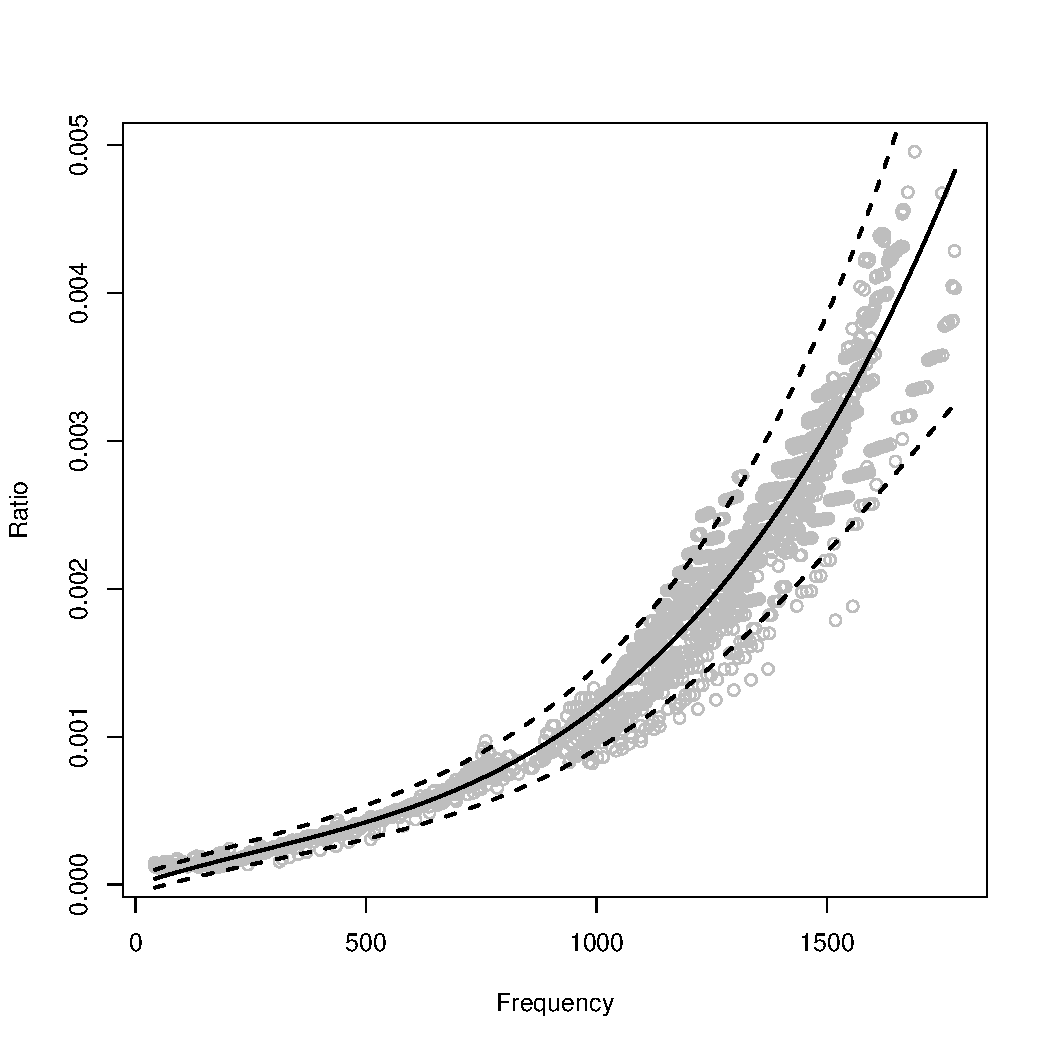
\includegraphics[width=0.45\textwidth]{plots/model}
 \caption{Ratio $M_{\rm PNS}/R_{\rm PNS}^2$ from our 18 1D simulations of the model set. The solid line is the maximum likelihood estimate of heteroscedastic cubic model with 95\% confidence bands (dashed lines) considering the 18 simulation data points. We have not made the distinction between the different simulations since we are only interested in the relationship between the variables.
 \pcd{[RATIO SHOULD BE MULTIPLIED BY A FACTOR 2 IN THE PLOT]}
 }
 \label{fig:LMVAR}
\end{figure}



\begin{table}[h]
 \begin{tabular}{crr}
    \hline
    Coefficient & \multicolumn{1}{c}{Estimate} & Standard error \\
    \hline
   $\beta_1$  &  $ 1.00 \times 10^{-06}$ & $2.12 \times 10^{-08}$ \\   
   $\beta_2$  &  $-8.22 \times 10^{-10}$ & $5.00 \times 10^{-11}$ \\
   $\beta_3$  &  $ 1.01 \times 10^{-12}$ & $2.70 \times 10^{-14}$ \\
   $\alpha_0$ &  $-1.02 \times 10^{+01}$ & $6.80 \times 10^{-02}$ \\
   $\alpha_1$ &  $ 7.24 \times 10^{-04}$ & $1.56 \times 10^{-04}$ \\
   $\alpha_2$ &  $ 6.23 \times 10^{-07}$ & $8.15 \times 10^{-08}$ \\   
    \hline
  \end{tabular}
\caption{Estimate and standard error of the coefficients of the best fit model describing the ratio $r=M_{\rm PNS}/R_{\rm PNS}^2$ as function of the frequency of the $\mbox{}^2g_2$ mode.\pcd{[CORRECT NUMBERS IN THE TABLE. JUST A FACTOR 2 iIN ALL COEFFICIENTS?]}}\label{tab:model}
\end{table}

\begin{figure}
 \centering
 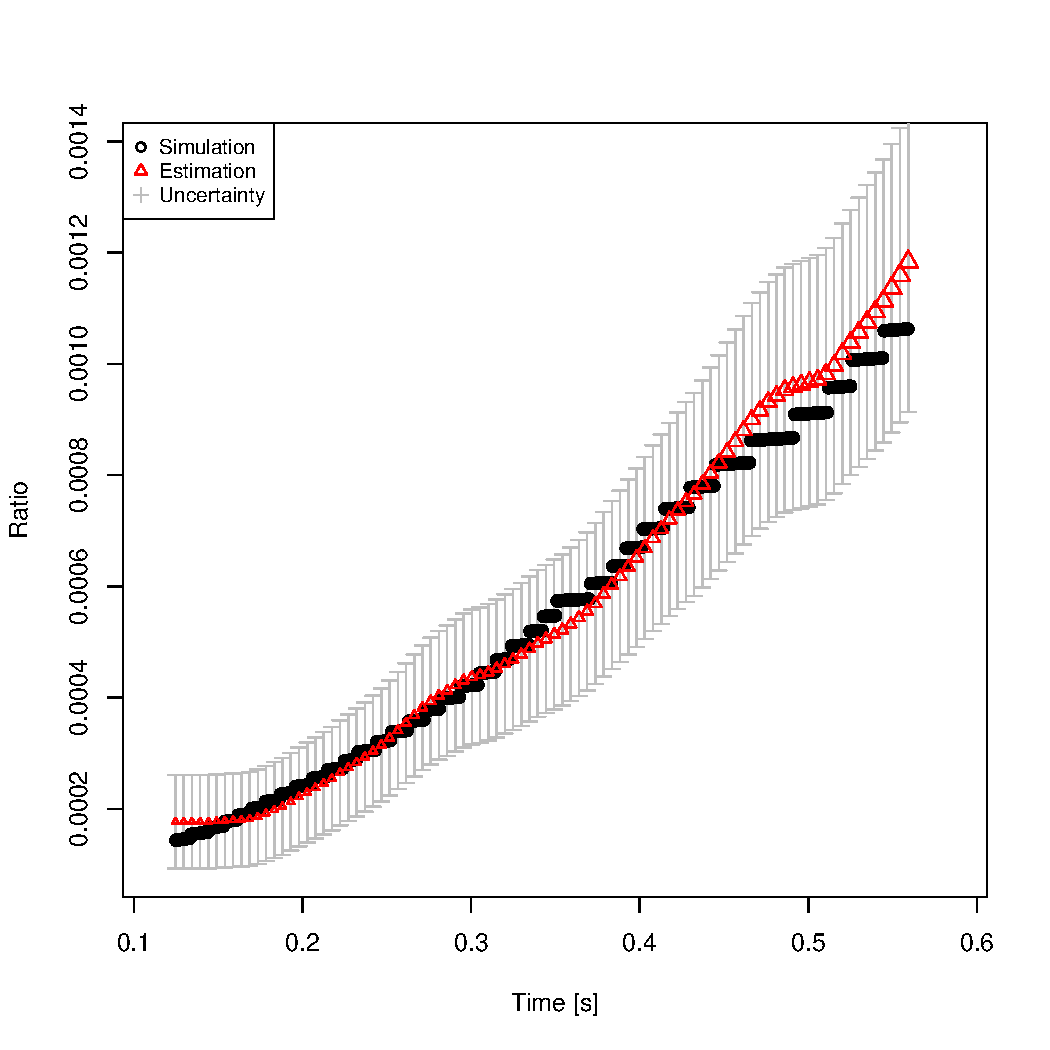
\includegraphics[width=0.5\textwidth]{plots/ratio}
 \caption{Comparison of the time evolution of the ratio $M_{\rm PNS}/R_{\rm PNS}^2$ estimated from the $\mbox{}^2 g_2$-mode of the {\texttt s20S} signal (shown by open triangles and by the 95\% confidence belt in grey) against the value derived from the PNS mass and radius given by the simulation code (shown by filled black circles). The size of the triangles are represented proportionally to the magnitude of the $\mbox{}^2 g_2$-mode frequency estimates. \pcd{[RATIO SHOULD BE MULTIPLIED BY A FACTOR 2 IN THE PLOT]}}
 \label{fig:ratio}
\end{figure}


\bibliographystyle{unsrt}
\bibliography{biblio}


\end{document}
